\chapter{Specific Requirements}

\section{External Interface Requirements}
\subsection{User Interfaces}

\begin{figure}[H]
    \centering
    \includegraphics[width=0.9\textwidth]{pdf/User_interfaces.pdf}
    \caption{User Interfaces Map}
    \label{fig:User_interfaces}
\end{figure}
\newpage
\noindent
The Best Bike Paths (BBP) User interface shall be designed to be intuitive and strictly adherent to a \emph{map-centric} approach, considering that the application will be used primarily on mobile devices in outdoor settings. The interactions shall be optimized for single-handed usage and high legibility while moving.


In compliance with \hyperref[standards-compliance]{accessibility requirements} and store guidelines, the interface shall use high-contrast colour schemes, scalable fonts, and enlarged touch targets to facilitate interaction during physical activity.

\noindent
The main System screens are described below:

\begin{itemize}
    \item \textbf{Landing Screen (Authentication)}: 
    Upon launching the app, the User is presented with a mandatory \emph{Safety Disclaimer} regarding road risks. Once acknowledged, the screen offers clear entry points:
        \begin{itemize}
            \item \emph{Log In / Sign Up}: Standard input fields for registered Users to access their profile.
            \item \emph{Continue as Guest}: A prominent, high-visibility button allowing immediate access to map exploration without account creation.
        \end{itemize}

    \item \textbf{Home Dashboard}: 
    The central hub of the application, existing in two distinct versions: \emph{Guest Mode} (with restricted features) and \emph{Registered Mode} (providing full access).
        \begin{itemize}
            \item \emph{Interactive Map}: The core interface element occupying the majority of the screen, displaying the User's real-time position and nearby cycling Paths colour-coded by their aggregated status (\eg, Green for Optimal, Red for Damaged).
            \item \emph{Search Bar}: Floating at the top, allowing quick entry of source and destination points.
            \item \emph{Start Recording}: A large Floating Action Button to begin a Trip, available exclusively in Registered Mode.
            \item \emph{Bottom Navigation Bar}: Provides quick access to \emph{Explore}, \emph{Profile} and, for registered Users only, \emph{My Activity} (with subsections for Trips/Paths).
        \end{itemize}

    \item \textbf{Profile Section}: 
    Manages global application preferences and User session state. The interface adapts its content based on whether the User is Registered or navigating as a Guest.
    \begin{itemize}
        \item \emph{App Settings}: Manages app-specific technical configurations and privacy controls. While sensor usage consent is available to all, specific identity management features (\eg, GDPR data export, Account Deletion) are hidden for Guest Users.
        \item \emph{Authentication Controls}: A dynamic area that manages the current session status.
        \begin{itemize}
            \item For \textbf{Registered Users}, it displays a \emph{Logout} button to terminate the session.
            \item For \textbf{Guest Users}, it displays \emph{Log In} and \emph{Sign Up} buttons (or a banner) to encourage account creation and unlock full features.
        \end{itemize}
    \end{itemize}
    
    \item \textbf{Explore}: Serving as the application's main page for navigation, this section is centered around the \emph{Interactive Map}, which allows Users to browse the cycling network directly. It also provides access to the search functionality, detailed as follows:
    \begin{itemize}
        \item \textbf{Search Routes \& Results}: Upon entering a source and destination, the interface presents \emph{Route Alternatives} via a list or map overlay showing possible routes. Each option highlights the \emph{Score} (calculated by the search algorithm) and the aggregated \emph{Status}, alongside \emph{Warnings} represented by icons indicating specific issues reported by the community (\eg, \emph{Muddy section}).
    \end{itemize}

    \item \textbf{My Activity}:
    This section is divided into two primary subsections:
    \begin{itemize}
        \item \textbf{My Trips Section}: Contains the chronological \emph{History List} of activities and the \emph{Trip Detail} view featuring graphs and maps, from which the \emph{Delete Trip} action can be performed. 
        \item \textbf{My Paths Section}: This section manages the repository of saved Paths, featuring a \emph{Path Library} that distinguishes between private and public entries. Users can access individual \emph{Path Details} to view metadata or execute the \emph{Delete Path} command to remove orphan Paths. 
        \begin{itemize} 
            \item \emph{Manual Path Creation}: Accessible here, it allows Users to define a Path without cycling via the \emph{Define Track} map editor and the \emph{Add Details} form for status and visibility. 
        \end{itemize}
    \end{itemize}

    \item \textbf{Recording Flow}:The tracking process is managed through two primary interfaces designed to minimize distraction and ensure data quality:
    \begin{itemize}
        \item \textbf{Active Recording Interface}: It is optimized for use while moving, displaying real-time metrics (speed, distance) and providing visual feedback for \emph{Auto-Pause} events. To prevent accidental interruptions during the ride, the \emph{Stop/Finish} function utilizes a deliberate ``slide-to-confirm'' interaction to terminate the session.
        \item Upon completion, the System presents the \textbf{Post-Ride Validation} screen, a critical summary for data aggregation displayed immediately after finishing a recording. In addition to presenting a final snapshot of performance statistics (duration, average speed) and the weather conditions automatically retrieved for the Trip's location , this interface allows the User to toggle the Path visibility between \emph{Private} and \emph{Public}  before finalizing the following data: 
        \begin{itemize} 
            \item \emph{Obstacle Validation}: A list allowing the User to confirm or reject anomalies automatically detected by the sensors. 
            \item \emph{Manual Obstacle Entry}: A specialized interaction allowing the User to manually drop a marker on the map to categorize obstacles that the automated sensors failed to detect during the ride.
            \item \emph{Path Rating}: A tool to assign a general status to the traversed Path (\eg, \emph{Optimal}). While this applies to all Segments by default, the User can override the status for specific map sections (\eg, marking a single stretch as \emph{Muddy}).
            \item \emph{Save/Delete Trip}: The final step to confirm saving the Trip to the database or permanently deleting the recording.
        \end{itemize}
    \end{itemize}
\end{itemize}

\subsection{Hardware Interfaces}
The BBP mobile application shall interact directly with specific hardware components embedded in the User's mobile device to fulfil its core functional requirements (tracking and sensing). The interactions are managed through the abstraction layers provided by the mobile operating System:

\begin{itemize}
    \item \textbf{Global Navigation Satellite System (GNSS) Receiver}:
    The application shall interface with the device's GPS/GNSS module to acquire real-time geospatial coordinates (latitude, longitude, altitude) and speed. The interface shall support background acquisition modes to allow Path recording while the screen is locked or the app is in the background.

    \item \textbf{Inertial Measurement Unit (IMU)}:
    To support the \emph{Automated Data Acquisition} and obstacle detection features, the application shall interface with the motion sensors:
    \begin{itemize}
        \item \textbf{Accelerometer}: To detect sudden vertical accelerations (shocks) indicative of potholes or irregular terrain.
        \item \textbf{Gyroscope}: To measure device orientation and rotation, helping to distinguish between a bicycle turning and random device movement.
    \end{itemize}

    \item \textbf{Network Interface Controller (Radio Modem)}:
    The application shall control the device's Wi-Fi and Cellular (4G/5G) signals to transmit data to the backend. The software shall detect the state of the hardware link to trigger the \emph{Store-and-Forward} mechanism when the signal is lost.

    \item \textbf{Non-Volatile Storage (Flash Memory)}:
    The application interfaces with the internal storage hardware to persist the local database and map cache, ensuring data integrity during offline operations.

    \item \textbf{Hosting Infrastructure (Server-Side)}:
    The backend components shall interface with the underlying server infrastructure (typically provided by a Cloud Service Provider via IaaS/PaaS) to access the necessary computational resources:
    \begin{itemize}
        \item \textbf{Processing Units (vCPU)}: To execute the heavy \emph{Data Aggregation} and \emph{Path Finding} algorithms. The infrastructure must support horizontal scaling (adding more nodes) to handle concurrent load peaks.
        \item \textbf{High-Throughput Storage}: Fast I/O storage interfaces are required for the Database Management System to perform rapid geospatial queries and write operations for incoming Trip logs.
        \item \textbf{Broadband Network Connection}: The server hardware must provide a high-bandwidth uplink to handle simultaneous data synchronization from thousands of mobile clients without bottlenecking.
    \end{itemize}
\end{itemize}

\subsection{Software Interfaces}
The BBP System interacts with various software components to function correctly across client and server environments:

\begin{itemize}
    \item \textbf{Mobile Operating Systems}: 
    The client application shall be compatible with modern mobile operating Systems to maximize User reach. Specifically:
    \begin{itemize}
        \item \textbf{Android}: Support for Android 10 (API level 29) and higher.
        \item \textbf{iOS}: Support for iOS 15 and higher.
    \end{itemize}
    The application interfaces directly with the OS SDKs to access low-level hardware services (Location Manager, Sensor Manager for accelerometer/gyroscope) and background processing tasks.

    \item \textbf{Database Management Systems (DBMS)}:
    \begin{itemize}
        \item \textbf{Server-Side (Backend)}: The System shall utilize a DBMS with native support for geospatial queries to efficiently store and index Path coordinates, Segments, and spatial metadata.
        \item \textbf{Client-Side (Local Cache)}: To support data caching and synchronization requirements, the mobile application shall interface with a local embedded database. This allows for the temporary persistence of Trip recordings and map tiles when network connectivity is unavailable.
    \end{itemize}

    \item \textbf{External APIs}:
    \begin{itemize}
        \item \textbf{Map Service Provider}: The System shall interface with an external mapping API to retrieve vector map tiles for visualization and graph data for routing algorithms.
        \item \textbf{Meteorological Service}: The System shall interface with a third-party Weather API to retrieve historical and current weather conditions based on the timestamp and geolocation of the recorded Trips.
    \end{itemize}

    \item \textbf{Development Framework Runtime}: 
    Since the application is developed as a cross-Platform solution, it shall rely on the specific runtime environment of the chosen framework to translate application logic into native OS commands.
\end{itemize}

\subsection{Communication Interfaces}
The BBP System shall rely on standard network protocols to ensure secure and efficient data exchange between the mobile client, the backend server, and external third-party services:
\begin{itemize}
    \item \textbf{Communication Protocols}:
    \begin{itemize}
        \item \textbf{Client-Server}: The mobile application shall communicate with the BBP backend via a RESTful API over HTTPS. This ensures that all API endpoints (\eg, for login, Trip upload, Path search) are accessed using a standardized, stateless architecture.
        \item \textbf{Server-External Services}: The backend shall interact with the Weather and Map providers using their respective public APIs, strictly over HTTPS to maintain the chain of trust and security.
    \end{itemize}

    \item \textbf{Data Serialization}:
        Data exchanged between the client and the server (\eg, User profiles, Trip coordinates, sensor metadata) shall be serialized in JSON format. This choice minimizes data payload size, critical for mobile Users with limited data plans, and ensures compatibility with modern development frameworks.

    \item \textbf{Security in Transit}:
    To comply with GDPR and protect sensitive geolocation data from interception (Man-in-the-Middle attacks), all network traffic shall be encrypted using TLS 1.2 or higher. Unencrypted HTTP traffic is strictly prohibited.

    \item \textbf{Synchronization Mechanism}:
    Given the constraint of intermittent network coverage (as defined in \hyperref[domain_assumptions]{Domain Assumptions}), the communication interface shall implement an Asynchronous Store-and-Forward pattern. When the device is offline, the communication layer shall queue API requests (\eg, \emph{Upload Trip}) in the local storage. A background \emph{Connectivity Manager} shall monitor the network status and automatically flushes the queue once a stable internet connection is re-established, ensuring no data is lost due to connectivity drops.
\end{itemize}

\section{Functional Requirements}

\subsection{Use Case Diagram}
\begin{figure}[ht]
    \centering
    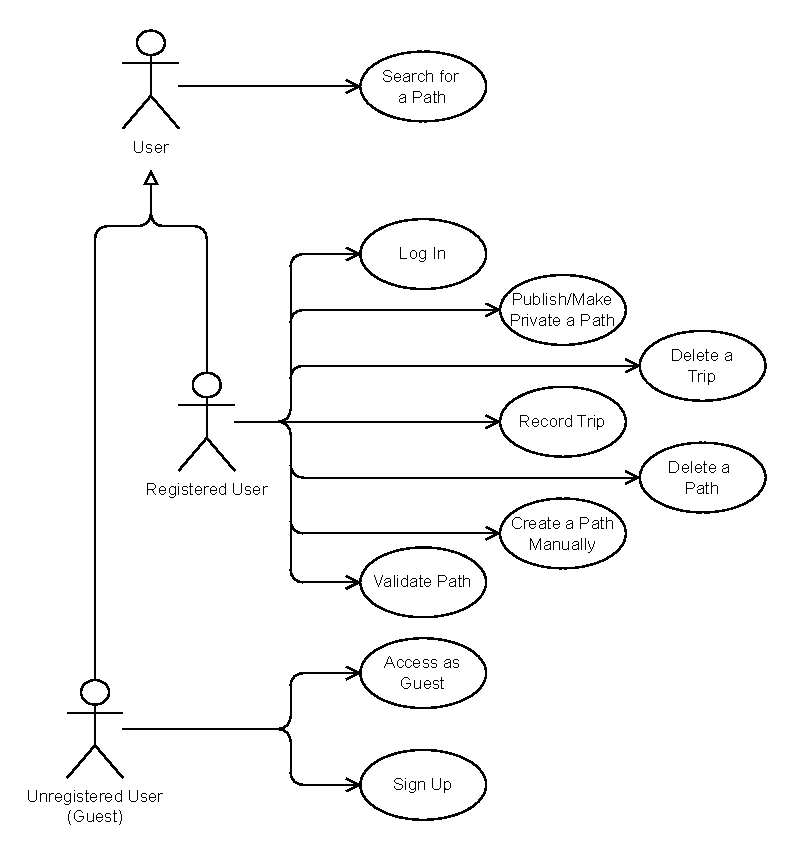
\includegraphics[width=\textwidth]{pdf/use_case_diagram.pdf}
    \caption{Use Case Diagram}
    \label{fig:use_case_diagram}
\end{figure}
\newpage
\subsection{Use Cases and Activity Diagrams}

\subsubsection*{[UC1] Sign Up by a User}
\begin{table}[H]
    \sf
    \small
    \centering
    \renewcommand{\arraystretch}{1.5}
    \begin{tabularx}{\textwidth}{|l|X|}
        \hline
        \cellcolor{lightgray} \textbf{Actor} & Unregistered User (Guest) \\
        \hline
        \cellcolor{lightgray} \textbf{Entry Conditions} & The User is not logged into the software. \\
        \hline
        \cellcolor{lightgray} \textbf{Flow of Events} & 
        \begin{enumerate}[leftmargin=*, before=\vspace*{-\baselineskip}]
            \item On the homepage, the User clicks the \emph{Sign Up} button, entering the initial registration page.
            \item The User provides the required details: name, surname and his other personal details, email, password and password confirmation.
            \item The User confirms the provided information by clicking the \emph{Register} button.
            \item The System verifies that the information is valid and that there is no existing profile associated with that email address.
            \item The System sends an OTP (One Time Password) to the email address provided to verify identity.
            \item The User enters the received OTP into the application.
            \item The System validates the OTP and activates the User's account.
            \item The User i redirected to the \emph{Explore} page.
        \end{enumerate}
        \\ 
        \hline
        \cellcolor{lightgray} \textbf{Exit Conditions} & The profile is complete and the User has access to its functionalities. \\
        \hline
        \cellcolor{lightgray} \textbf{Exceptions} & 
        \begin{itemize}[leftmargin=*, before=\vspace*{-\baselineskip}]
            \item Existing profile: If the email address provided is already associated with an account, the System will deny registration and inform the User.
            \item OTP verification failed: If the OTP entered is incorrect or does not match, the identity is not verified and the account is not activated until a correct one is provided (implicit in the verification process).
        \end{itemize}
        \\ 
        \hline
    \end{tabularx}
    \caption{UC1: Sign Up by a User}
\end{table}
\newpage
\begin{figure}[H]
    \centering
    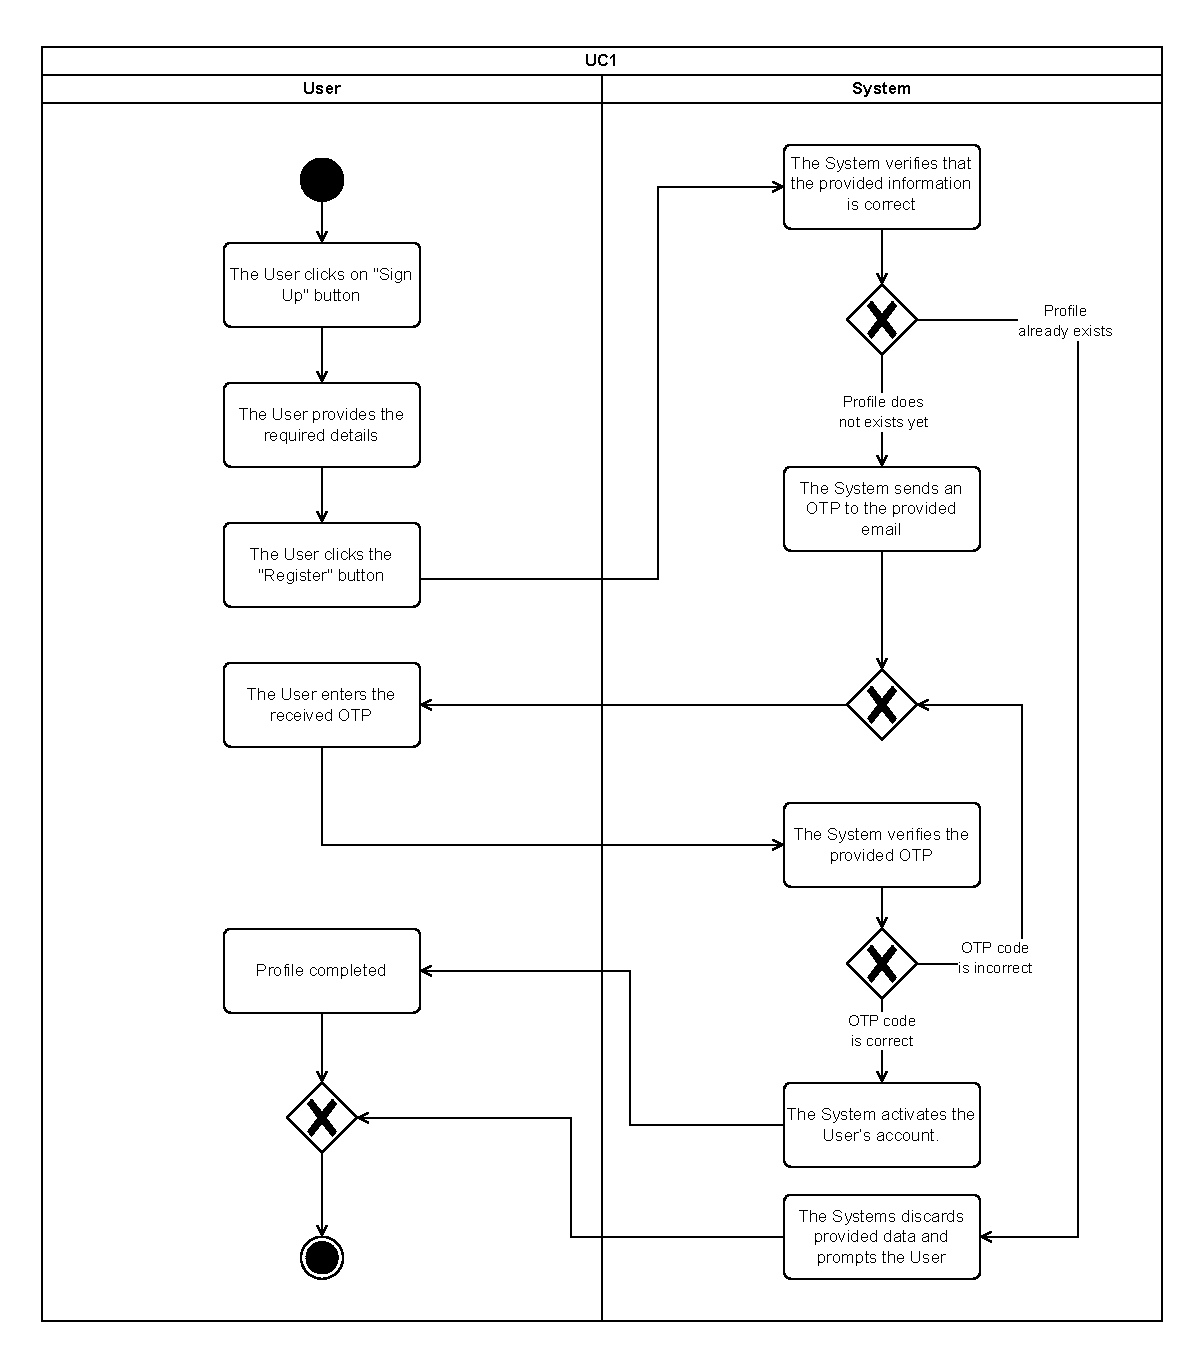
\includegraphics[width=\textwidth]{pdf/UC1.pdf}
    \caption{UC1 Activity Diagram}
    \label{fig:UC1}
\end{figure}
\newpage
\subsubsection*{[UC2] Log In by a User}
\begin{table}[H]
    \sf
    \small
    \centering
    \renewcommand{\arraystretch}{1.5}
    \begin{tabularx}{\textwidth}{|l|X|}
        \hline
        \cellcolor{lightgray} \textbf{Actor} & Registered User \\ 
        \hline
        \cellcolor{lightgray} \textbf{Entry Conditions} & The User is not already logged into the software. \\ 
        \hline
        \cellcolor{lightgray} \textbf{Flow of Events} & 
        \begin{enumerate}[leftmargin=*, before=\vspace*{-\baselineskip}]
            \item On the homepage, the User clicks the \emph{Login} button, which displays the login form.
            \item The User enters their email and password into the designated fields.
            \item The User clicks the \emph{Login} button.
            \item The System validates the provided credentials.
            \item The System redirects the User to the \emph{Explore} page.
        \end{enumerate}
        \\ 
        \hline
        \cellcolor{lightgray} \textbf{Exit Conditions} & The User is successfully logged in. \\ 
        \hline
        \cellcolor{lightgray} \textbf{Exceptions} & 
        \begin{itemize}[leftmargin=*, before=\vspace*{-\baselineskip}]
            \item Incorrect credentials: If the credentials provided are incorrect, the System denies access and prompts the User to try again.
        \end{itemize}
        \\ 
        \hline
    \end{tabularx}
    \caption{UC2: Log In by a User}
\end{table}
\newpage
\begin{figure}[H]
    \centering
    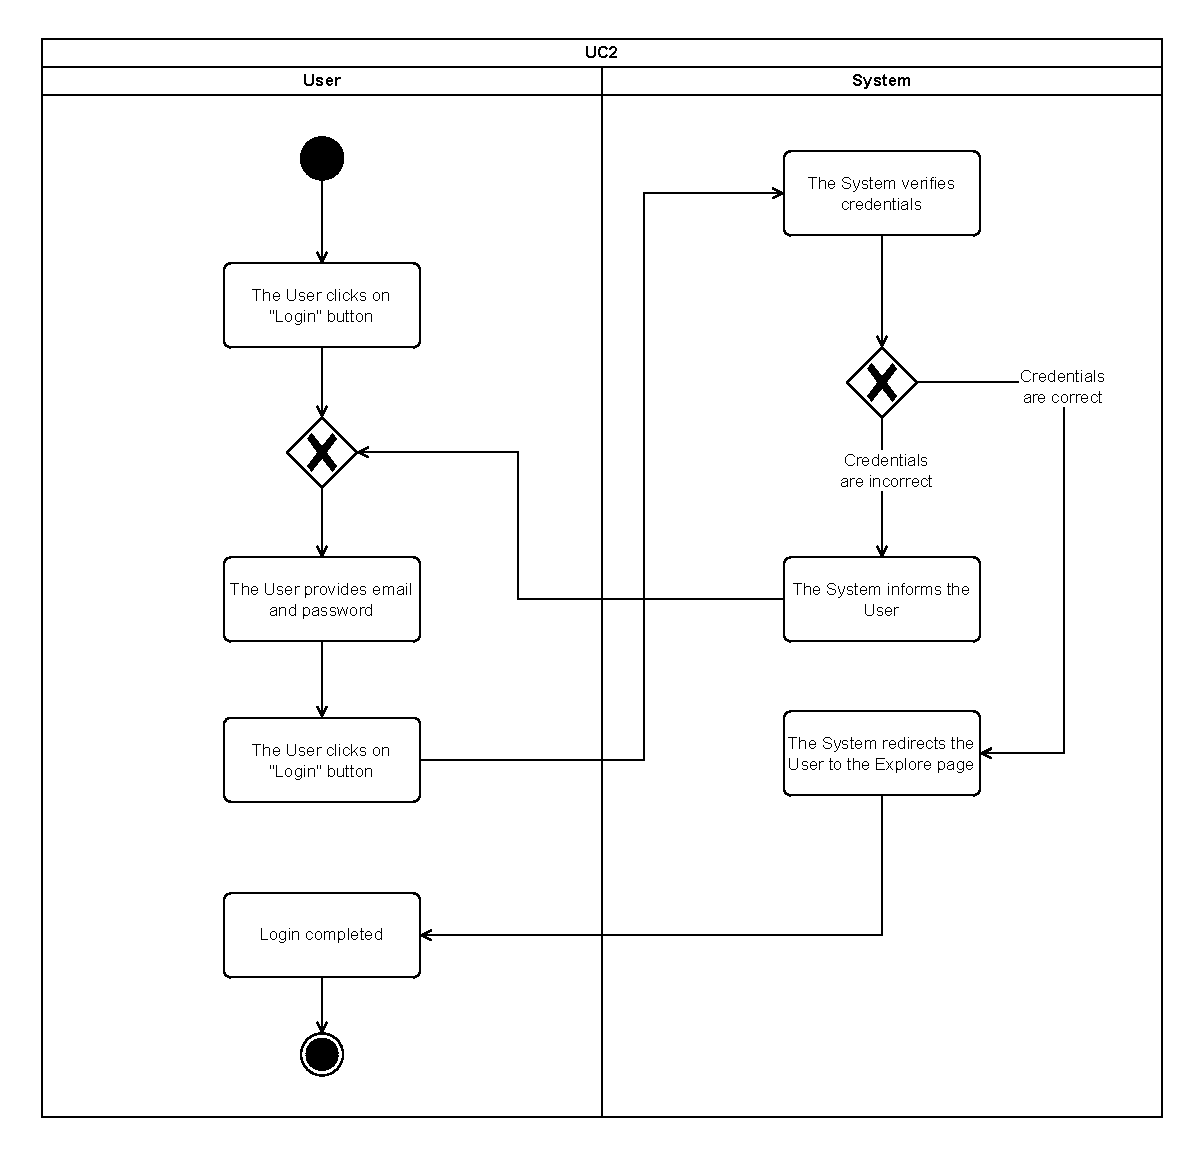
\includegraphics[width=\textwidth]{pdf/UC2.pdf}
    \caption{UC2 Activity Diagram}
    \label{fig:UC2}
\end{figure}
\newpage
\subsubsection*{[UC3] Access as Guest}
\begin{table}[H]
    \sf
    \small
    \centering
    \renewcommand{\arraystretch}{1.5}
    \begin{tabularx}{\textwidth}{|l|X|}
        \hline
        \cellcolor{lightgray} \textbf{Actor} & Unregistered User (Guest) \\ 
        \hline
        \cellcolor{lightgray} \textbf{Entry Conditions} & The User has opened the application and is on the landing screen. \\ 
        \hline
        \cellcolor{lightgray} \textbf{Flow of Events} & 
        \begin{enumerate}[leftmargin=*, before=\vspace*{-\baselineskip}]
            \item On the Login/Sign Up screen, the User selects the \emph{Continue as Guest} option.
            \item The System grants access to the public features of the application (Search, Map Visualization).
            \item The System restricts access to private features (Recording, My Activity) by hiding them or disabling the buttons.
            \item The User is redirected to the \emph{Explore} page.
        \end{enumerate}
        \\ 
        \hline
        \cellcolor{lightgray} \textbf{Exit Conditions} & The User can browse and search for Paths but cannot record data. \\ 
        \hline
    \end{tabularx}
    \caption{UC3: Access as Guest}
\end{table}
\newpage
\begin{figure}[H]
    \centering
    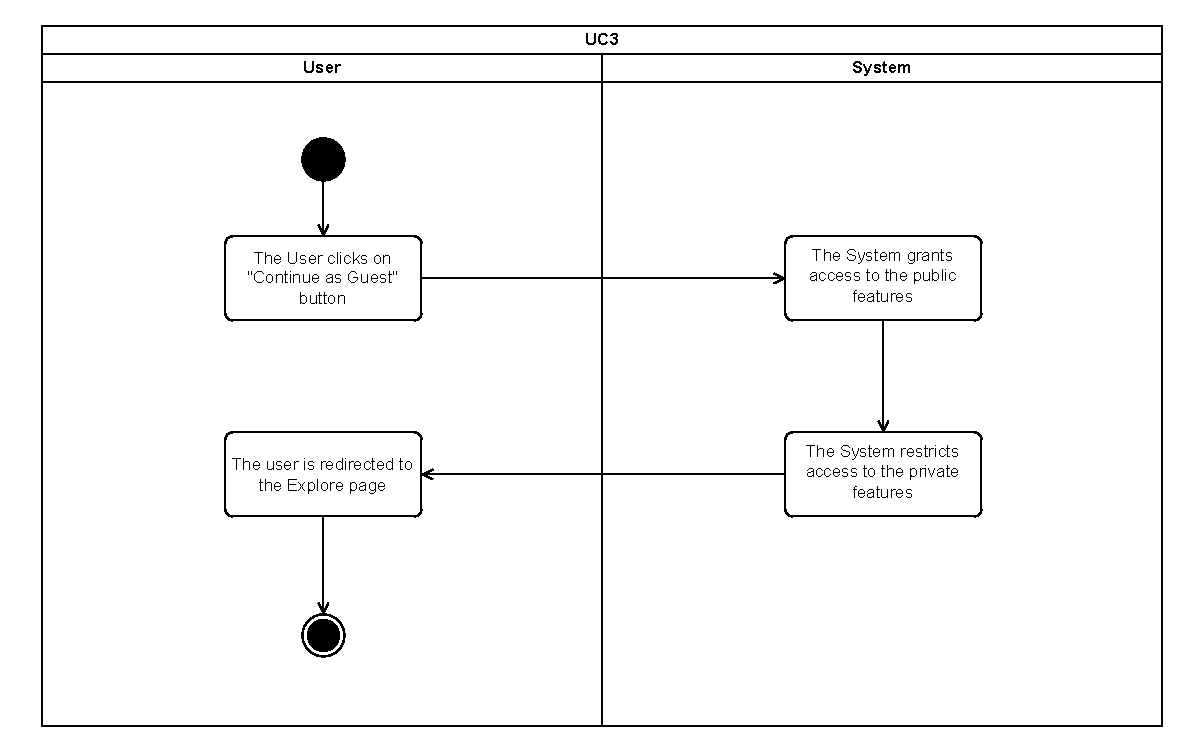
\includegraphics[width=\textwidth]{pdf/UC3.pdf}
    \caption{UC3 Activity Diagram}
    \label{fig:UC3}
\end{figure}
\newpage
\subsubsection*{[UC4] Record a Trip}
\begin{table}[H]
    \sf
    \small
    \centering
    \renewcommand{\arraystretch}{1.5}
    \begin{tabularx}{\textwidth}{|l|X|}
        \hline
        \cellcolor{lightgray} \textbf{Actor} & Registered User \\ 
        \hline
        \cellcolor{lightgray} \textbf{Entry Conditions} & The User is logged into the software. \\ 
        \hline
        \cellcolor{lightgray} \textbf{Flow of Events} & 
        \begin{enumerate}[leftmargin=*, before=\vspace*{-\baselineskip}]
            \item The User selects the \emph{Start Cycling} command to begin a session.
            \item The System automatically begins recording GPS coordinates to track the Path.
            \item While cycling, the System analyses accelerometer and gyroscope data to automatically detect potential obstacles (\eg, potholes).
            \item If the System detects that the User's speed drops below a threshold or movement indicates walking, it automatically pauses data acquisition.
            \item The System automatically resumes recording when the User starts pedalling again.
            \item The User selects the \emph{End Cycling} command to end the session.
            \item The System retrieves weather data from an external service associated with the location and time of the Trip.
            \item The System calculates performance statistics (speed, duration, distance).
            \item The System presents a Trip summary and prompts the User to validate any detected obstacles.
        \end{enumerate}
        \\ 
        \hline
        \cellcolor{lightgray} \textbf{Exit Conditions} & The Trip has been recorded, the statistics are calculated, and the Path is ready for User validation. \\ 
        \hline
        \cellcolor{lightgray} \textbf{Exceptions} & 
        \begin{itemize}[leftmargin=*, before=\vspace*{-\baselineskip}]
            \item Non-Cycling Activity: If the User never cycles (\eg, only walks), the System pauses recording and the Segment is not added to the cycling Path inventory.
        \end{itemize}
        \\ 
        \hline
    \end{tabularx}
    \caption{UC4: Record a Trip}
\end{table}
\newpage
\begin{figure}[H]
    \centering
    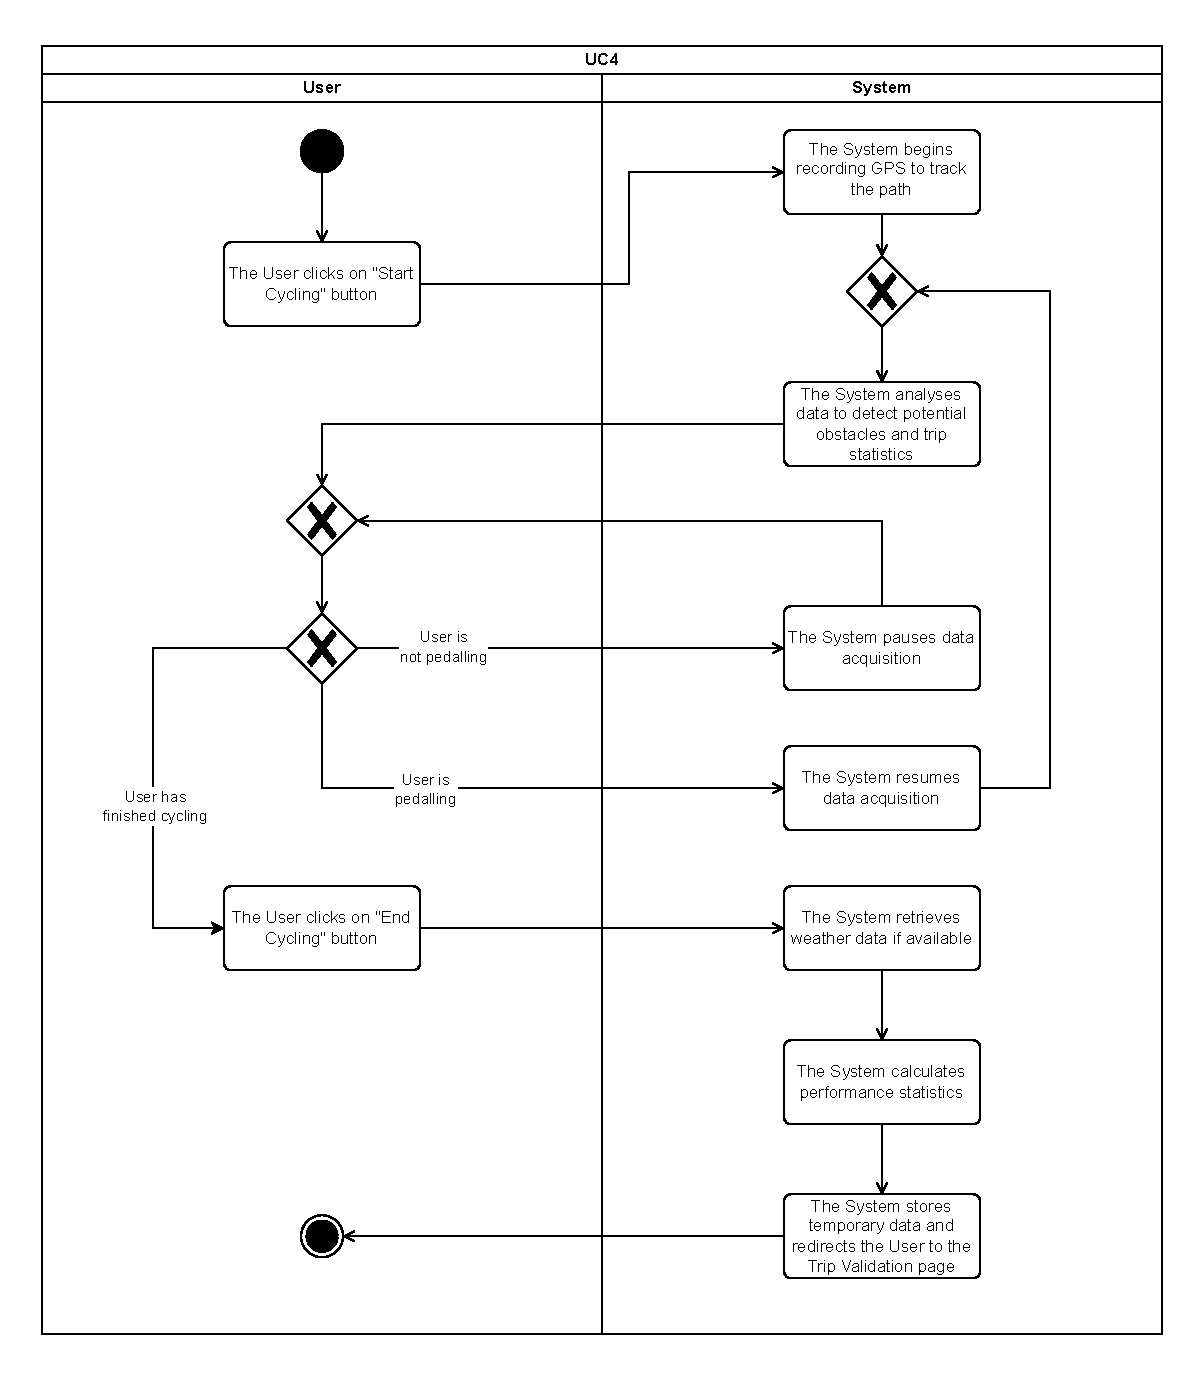
\includegraphics[width=\textwidth]{pdf/UC4.pdf}
    \caption{UC4 Activity Diagram}
    \label{fig:UC4}
\end{figure}
\newpage
\subsubsection*{[UC5] Validate a Trip and Path}
\begin{table}[H]
    \sf
    \small
    \centering
    \renewcommand{\arraystretch}{1.5}
    \begin{tabularx}{\textwidth}{|l|X|}
        \hline
        \cellcolor{lightgray} \textbf{Actor} & Registered User \\ 
        \hline
        \cellcolor{lightgray} \textbf{Entry Conditions} & The User is logged into the software and they have just finished a recording session (pressed \emph{End Cycling}). \\ 
        \hline
        \cellcolor{lightgray} \textbf{Flow of Events} & 
        \begin{enumerate}[leftmargin=*, before=\vspace*{-\baselineskip}]
            \item The System shows the User a Trip summary and any automatically detected obstacles.
            \item The User examines the proposed obstacles.
            \item The User confirms the presence of real obstacles or rejects false positives (swiping or tapping on the list).
            \item The User manually inserts any additional obstacles that the System failed to detect, pinpointing them on the map and assigning a type (\eg, \emph{Pothole}).
            \item The User assigns a general status to the Path just completed (\eg, \emph{Optimal,} \emph{Needs Maintenance}).
            \item The System applies this status to all the road Segments traversed during the Trip and,         \item Optionally, the User selects specific Segments on the map to override the general status with a more specific one (\eg, marking only one section as \emph{Needs Maintenance}).
            \item The User confirms saving the Trip and the Path and decides whether to make the Path public or private.
            \item The System permanently saves the Trip, the Path (linking the specific Segment statuses) and confirmed data in the database, preventing future changes to the GPS track. If the User opted for the publication of the Path, the System launches the aggregation algorithm: it recalculates the status of the affected road Segments by merging the User's new data with the community's existing data.
        \end{enumerate}
        \\ 
        \hline
        \cellcolor{lightgray} \textbf{Exit Conditions} & The Trip is saved and the Path is validated and saved in the User's profile; the obstacle information has been cleaned of false positives.\\ 
        \hline
        \cellcolor{lightgray} \textbf{Exceptions} & 
        \begin{itemize}[leftmargin=*, before=\vspace*{-\baselineskip}]
            \item Trip cancellation: If the User realizes that the recording is invalid, they decide to delete the entire Trip (Path included) instead of validating it. The System removes all temporary data and nothing is saved.
        \end{itemize}
        \\ 
        \hline
    \end{tabularx}
    \caption{UC5: Validate a Trip and Path}
\end{table}
\newpage
\begin{figure}[H]
    \centering
    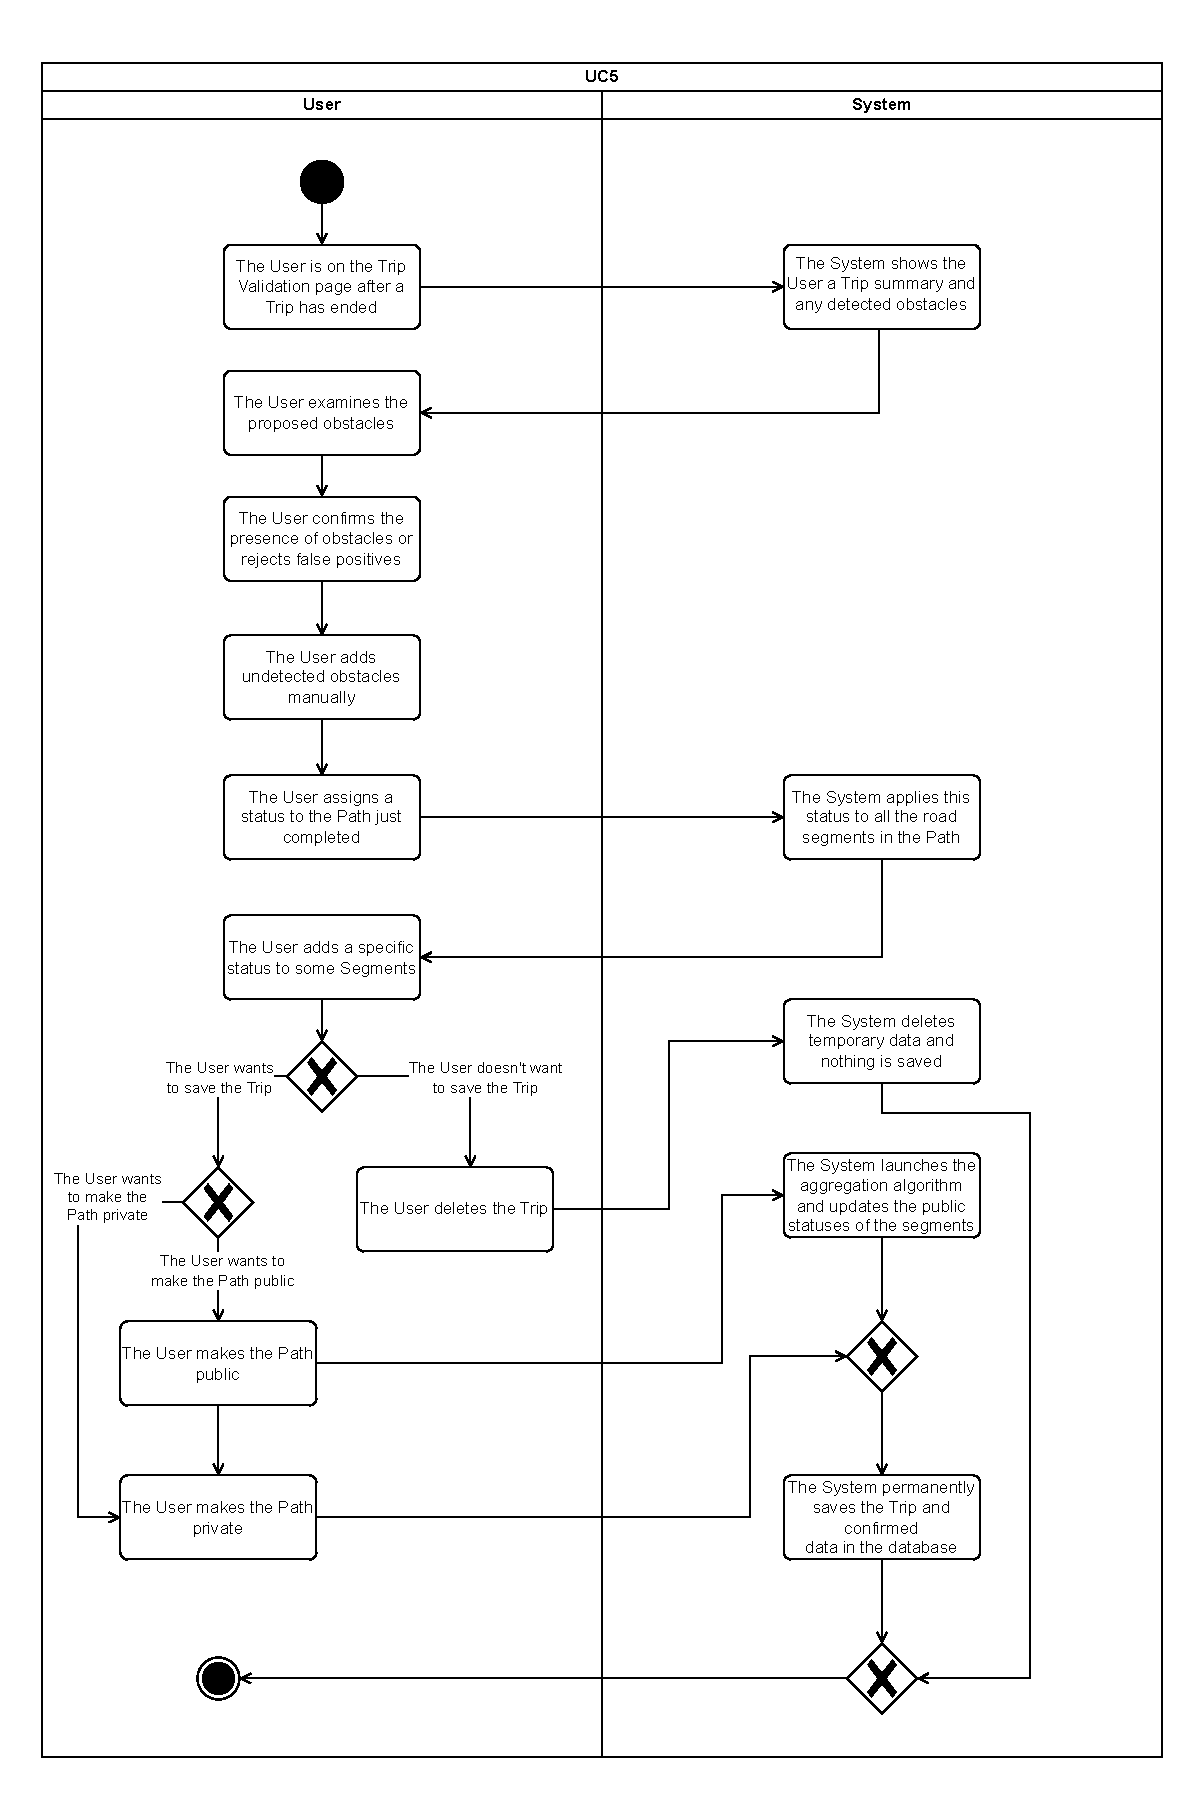
\includegraphics[width=\textwidth]{pdf/UC5.pdf}
    \caption{UC5 Activity Diagram}
    \label{fig:UC5}
\end{figure}
\newpage
\subsubsection*{[UC6] Change Path's visibility}
\begin{table}[H]
    \sf
    \small
    \centering
    \renewcommand{\arraystretch}{1.5}
    \begin{tabularx}{\textwidth}{|l|X|}
        \hline
        \cellcolor{lightgray} \textbf{Actor} & Registered User \\ 
        \hline
        \cellcolor{lightgray} \textbf{Entry Conditions} & The User has inserted a Path, either manually or automatically, and is in the Path details page. \\ 
        \hline
        \cellcolor{lightgray} \textbf{Flow of Events} & 
        \begin{enumerate}[leftmargin=*, before=\vspace*{-\baselineskip}]
            \item The User chooses the option to make the Path \emph{Public}.
            \item The System receives the request and updates the Path's visibility attribute.
            \item The System launches the aggregation algorithm: it recalculates the status of the affected road Segments by merging the User's new data with the community's existing data.
            \item The System resolves any data conflicts based on the freshness of the information and the number of confirmed reports.
            \item The System confirms to the User that the Path has been successfully published.
        \end{enumerate}
        \\ 
        \hline
        \cellcolor{lightgray} \textbf{Exit Conditions} & The Path is visible to all Users on the global map and aggregated community data (scores, road status) has been updated.\\ 
        \hline
        \cellcolor{lightgray} \textbf{Exceptions} & The Path was already public: the System will not perform any operation.\\
        \hline
    \end{tabularx}
    \caption{UC6: Change of Path's visibility}
\end{table}
Note that the described procedure outlines the process for making a Path public. However, it is also possible to revert a previously published Path to a private state in the same way. In such a case, the System would set the visibility status to \emph{private} and all related aggregated data would be restored.
\newpage
\begin{figure}[H]
    \centering
    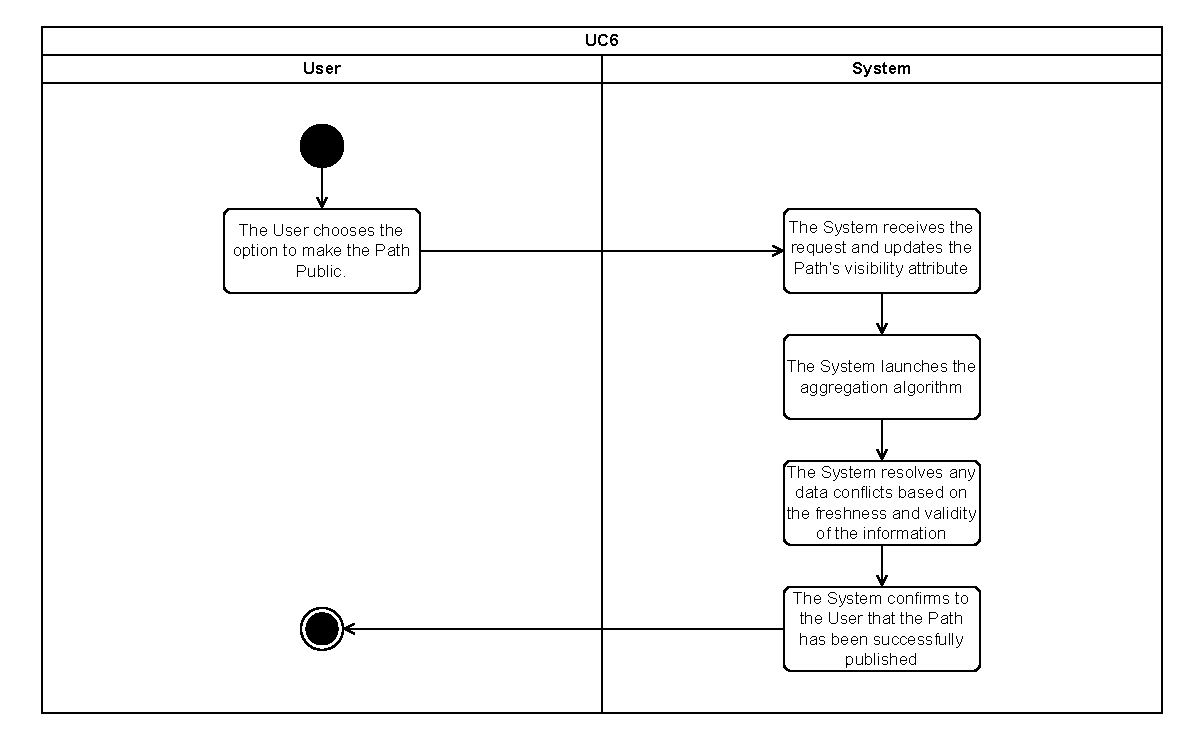
\includegraphics[width=\textwidth]{pdf/UC6.pdf}
    \caption{UC6 Activity Diagram}
    \label{fig:UC6}
\end{figure}
\newpage
\subsubsection*{[UC7] Create a Path manually}
\begin{table}[H]
    \sf
    \small
    \centering
    \renewcommand{\arraystretch}{1.5}
    \begin{tabularx}{\textwidth}{|l|X|}
        \hline
        \cellcolor{lightgray} \textbf{Actor} & Registered User \\ 
        \hline
        \cellcolor{lightgray} \textbf{Entry Conditions} & The User is logged into the software and they have selected the \emph{Create a Path} functionality.\\ 
        \hline
        \cellcolor{lightgray} \textbf{Flow of Events} & 
        \begin{enumerate}[leftmargin=*, before=\vspace*{-\baselineskip}]
            \item The User interacts with the map and manually enters the sequence of road Segments connecting an entry and exit point.
            \item The User assigns a general status to the Path (\eg, \emph{Optimal}, \emph{Hard}) to warn future cyclists.
            \item The System applies this status to all selected Segments.
            \item Optionally, the User selects specific Segments on the map to override the general status with a more specific one (\eg, marking only one section as \emph{Needs Maintenance}).
            \item The User sets the Path visibility (public/private).
            \item The User confirms Path creation.
            \item The System validates that a list of roads and statuses has been provided.
            \item The System saves the Path in the database.
            \item If set to public, the System immediately updates the global map by recalculating the aggregated status of the involved Segments.
        \end{enumerate}
        \\ 
        \hline
        \cellcolor{lightgray} \textbf{Exit Conditions} & The new Path has been saved in the System and, if public, is integrated into the global inventory of cycling Paths.\\ 
        \hline
        \cellcolor{lightgray} \textbf{Exceptions} & 
        \begin{itemize}[leftmargin=*, before=\vspace*{-\baselineskip}]
            \item Incomplete Data: If the User attempts to save without providing the road list or status, the System prevents saving and requests the missing data.
            \item Mapping Error: If the selected Segments are not contiguous or valid on the map, the System reports a tracking error.
        \end{itemize}
        \\ 
        \hline
    \end{tabularx}
    \caption{UC7: Create a Path manually}
\end{table}
\newpage
\begin{figure}[H]
    \centering
    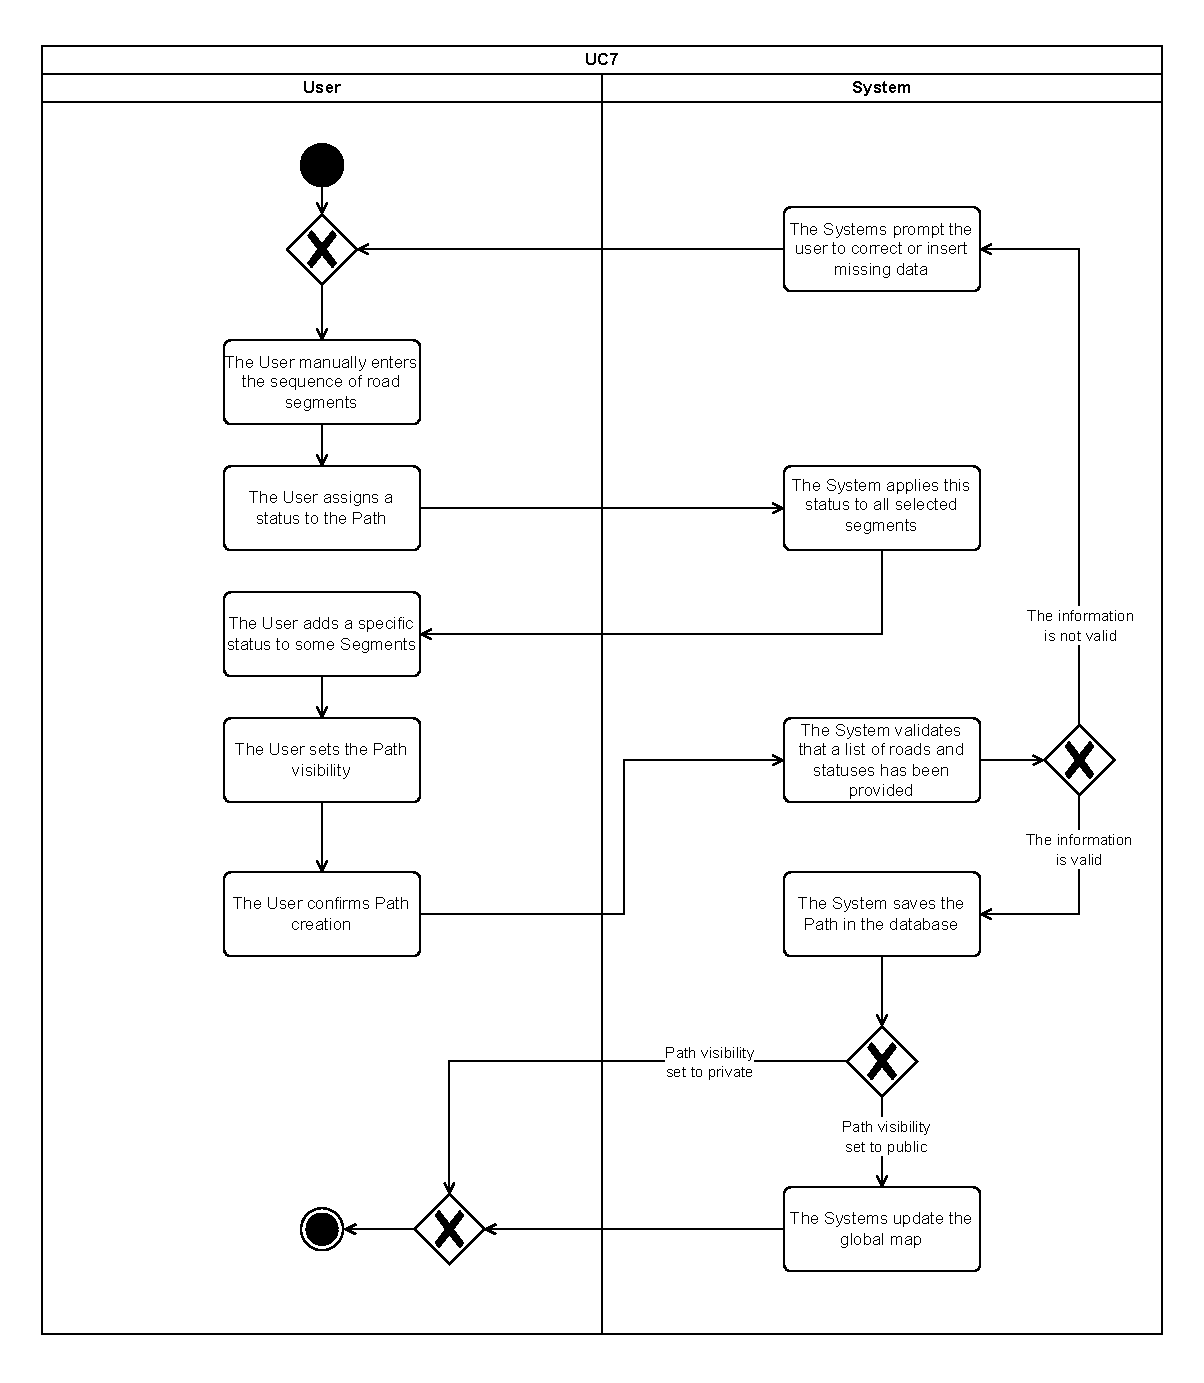
\includegraphics[width=\textwidth]{pdf/UC7.pdf}
    \caption{UC7 Activity Diagram}
    \label{fig:UC7}
\end{figure}
\newpage
\subsubsection*{[UC8] Search for a route}
\begin{table}[H]
    \sf
    \small
    \centering
    \renewcommand{\arraystretch}{1.5}
    \begin{tabularx}{\textwidth}{|l|X|}
        \hline
        \cellcolor{lightgray} \textbf{Actor} & Guest User, Registered User \\ 
        \hline
        \cellcolor{lightgray} \textbf{Entry Conditions} & The User has access to the application and they have selected the search section. \\ 
        \hline
        \cellcolor{lightgray} \textbf{Flow of Events} & 
        \begin{enumerate}[leftmargin=*, before=\vspace*{-\baselineskip}]
            \item The User enters a source point in the search form.
            \item The User enters a destination point in the search form.
            \item The System searches the database for possible routes connecting the two points.
            \item If multiple routes exist, the System calculates a score for each, based on the aggregate status (\eg, presence of potholes) and the efficiency/distance to the destination.
            \item The System displays the results on a map, sorting or filtering them based on the calculated score.
            \item The User views the alternatives and selects one for details.
        \end{enumerate}
        \\ 
        \hline
        \cellcolor{lightgray} \textbf{Exit Conditions} & The User sees a list of valid routes between the specified points, with their statuses and scores.\\ 
        \hline
        \cellcolor{lightgray} \textbf{Exceptions} & 
        \begin{itemize}[leftmargin=*, before=\vspace*{-\baselineskip}]
            \item No route found: If there are no mapped cycling routes between the origin and destination (or if they are not connected), the System informs the User that a route cannot be found.
        \end{itemize}
        \\ 
        \hline
    \end{tabularx}
    \caption{UC8: Search for a route}
\end{table}
\newpage
\begin{figure}[H]
    \centering
    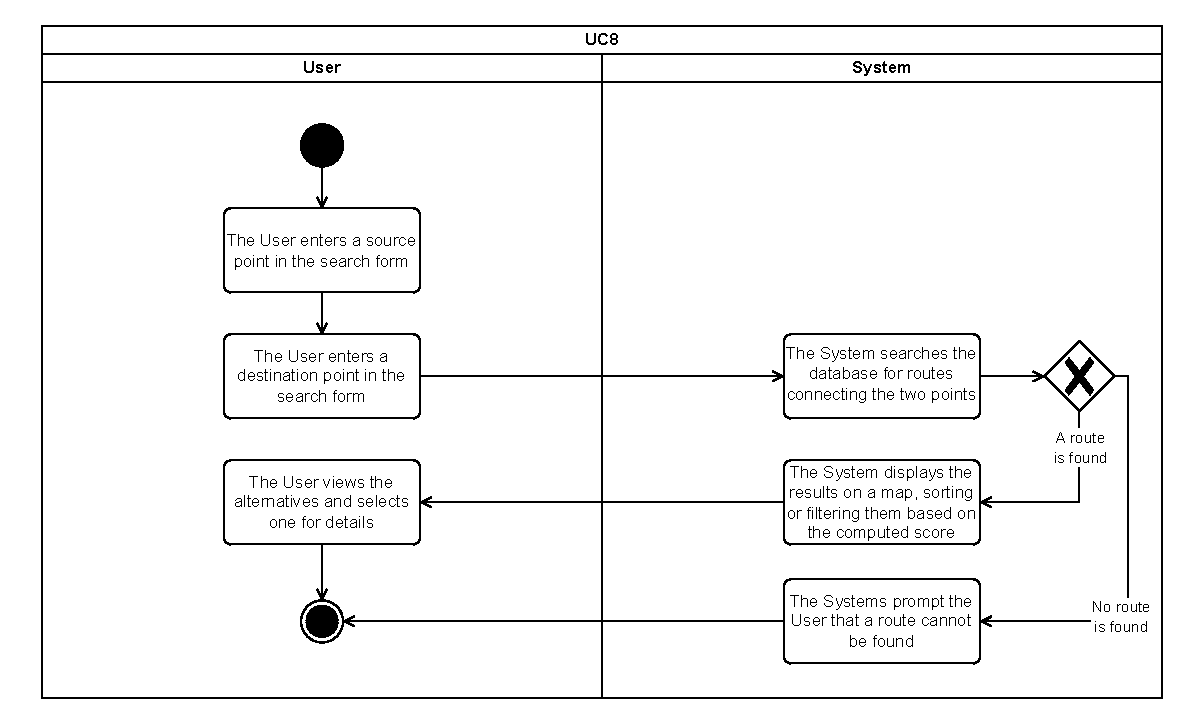
\includegraphics[width=\textwidth]{pdf/UC8.pdf}
    \caption{UC8 Activity Diagram}
    \label{fig:UC8}
\end{figure}
\newpage
\subsubsection*{[UC9] Delete a Trip}
\begin{table}[H]
    \sf
    \small
    \centering
    \renewcommand{\arraystretch}{1.5}
    \begin{tabularx}{\textwidth}{|l|X|}
        \hline
        \cellcolor{lightgray} \textbf{Actor} & Registered User \\ 
        \hline
        \cellcolor{lightgray} \textbf{Entry Conditions} & The User is logged in and has at least one recorded Trip in the \emph{My Trips} section. \\ 
        \hline
        \cellcolor{lightgray} \textbf{Flow of Events} & 
        \begin{enumerate}[leftmargin=*, before=\vspace*{-\baselineskip}]
            \item The User views the details of a specific Trip.
            \item The User presses the \emph{Delete} button.
            \item The System asks the User to choose the scope of the deletion:
                \begin{itemize}
                    \item Option A: Delete the Trip (statistics, time) but keep the Path (geometry/map).
                    \item Option B: Delete both the Trip and the associated Path.
                \end{itemize}
            \item The User selects an option and confirms the action.
            \item \textbf{Case A (Keep Path):} The System removes the Trip data (speed, duration) but retains the Path in the User's \emph{My Paths} list as a manually saved Path.
            \item \textbf{Case B (Delete Both):} The System removes both the Trip and the Path. If the Path was public, the System removes the User's contribution from the aggregated community data.
        \end{enumerate}
        \\ 
        \hline
        \cellcolor{lightgray} \textbf{Exit Conditions} & The Trip is removed. The associated Path is either preserved as an orphan entry or permanently deleted based on User choice. \\ 
        \hline
        \cellcolor{lightgray} \textbf{Exceptions} &
        \begin{itemize}[leftmargin=*, before=\vspace*{-\baselineskip}]
            \item User Cancellation: If the User cancels the confirmation prompt, no data is modified.
        \end{itemize}
        \\ 
        \hline
    \end{tabularx}
    \caption{UC9: Delete a Trip}
\end{table}
\newpage
\begin{figure}[H]
    \centering
    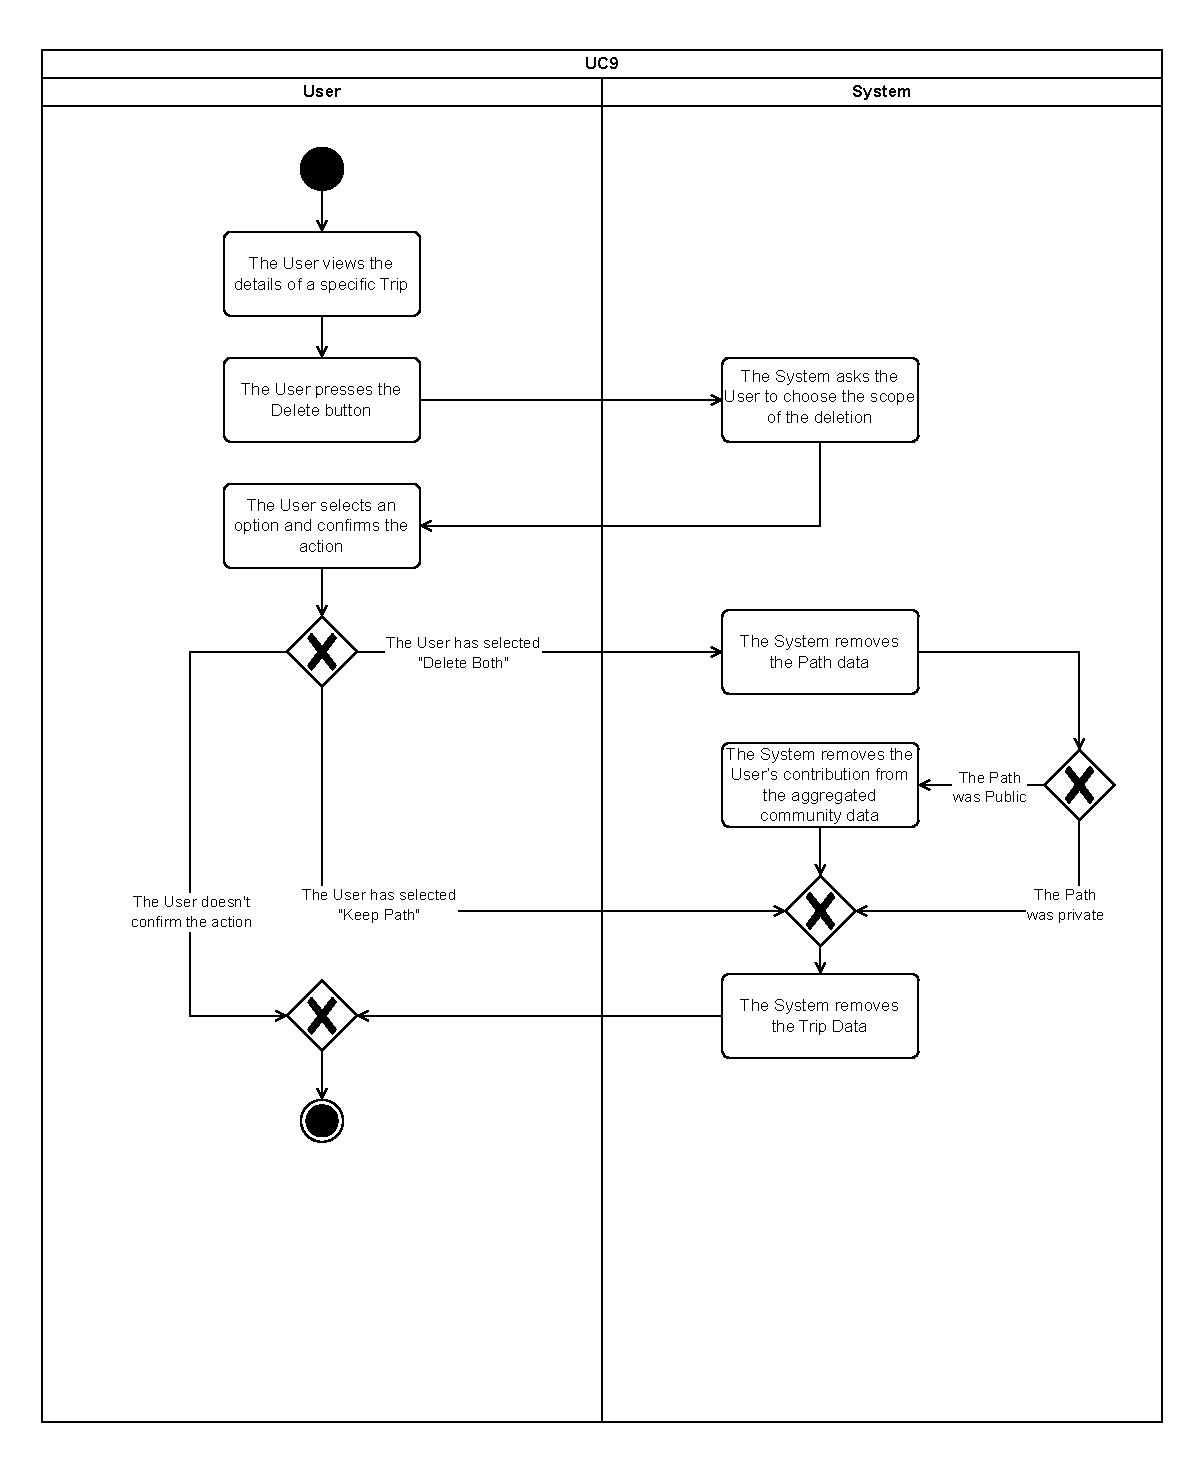
\includegraphics[width=\textwidth]{pdf/UC9.pdf}
    \caption{UC9 Activity Diagram}
    \label{fig:UC9}
\end{figure}
 \newpage
\subsubsection*{[UC10] Delete a Path}
\begin{table}[H]
    \sf
    \small
    \centering
    \renewcommand{\arraystretch}{1.5}
    \begin{tabularx}{\textwidth}{|l|X|}
        \hline
        \cellcolor{lightgray} \textbf{Actor} & Registered User \\ 
        \hline
        \cellcolor{lightgray} \textbf{Entry Conditions} & The User is logged in and has at least one Path in the \emph{My Paths} section. \\ 
        \hline
        \cellcolor{lightgray} \textbf{Flow of Events} & 
        \begin{enumerate}[leftmargin=*, before=\vspace*{-\baselineskip}]
            \item The User selects the specific Path they wish to remove.
            \item The User presses the \emph{Delete} button.
            \item The System checks for dependencies: it verifies if there is any existing recorded \emph{Trip} currently linked to this \emph{Path}.
            \item If no dependencies are found (the Path is \emph{orphan} or manually created), the System prompts for confirmation.
            \item The User confirms the operation.
            \item The System permanently removes the Path from the User's profile.
            \item If the Path was public, the System triggers the aggregate data update process to remove this contribution.
        \end{enumerate}
        \\ 
        \hline
        \cellcolor{lightgray} \textbf{Exit Conditions} & The Path is deleted from the System and removed from the global map aggregation if it was public. \\ 
        \hline
        \cellcolor{lightgray} \textbf{Exceptions} & 
        \begin{itemize}[leftmargin=*, before=\vspace*{-\baselineskip}]
            \item Dependency Error: If the System finds a \emph{Trip} associated with the Path, it blocks the deletion and displays an error message.
            \item User Cancellation: If the User denies confirmation, the Path remains intact.
        \end{itemize}
        \\ 
        \hline
    \end{tabularx}
    \caption{UC10: Delete a Path}
\end{table}
\newpage
\begin{figure}[H]
    \centering
    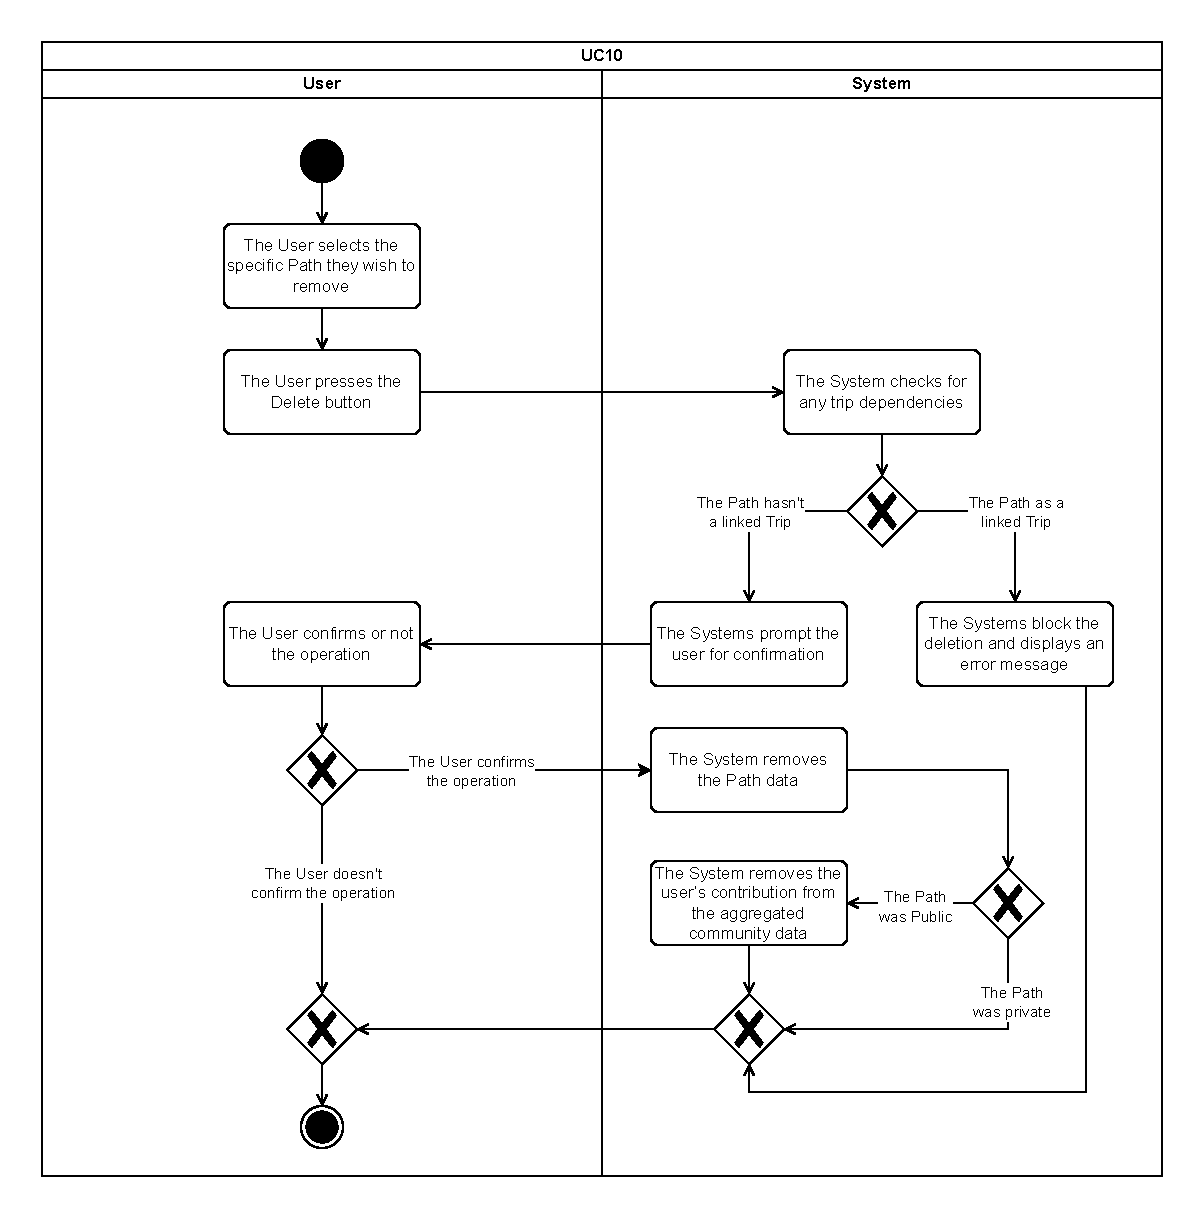
\includegraphics[width=\textwidth]{pdf/UC10.pdf}
    \caption{UC10 Activity Diagram}
    \label{fig:UC10}
\end{figure}
\newpage
\subsection{Requirement Mapping}
\begin{table}[H]
    \sf
    \small
    \centering
    \renewcommand{\arraystretch}{1.5}
    \begin{tabularx}{0.99\textwidth}{|l|X|X|X|}
        \hline
        \rowcolor{lightgray}
        \textbf{UC ID} & \textbf{Goals} & \textbf{Requirements} & \textbf{Assumptions} \\ \hline

        \textbf{UC1} & G2, G4, G8 & R1 & DA3, DA10 \\ \hline

        \textbf{UC2} & G1, G2, G3, G4, G5, G8 & R2 & DA10 \\ \hline

        \textbf{UC3} & G6, G7 & R3 & DA10 \\ \hline

        \textbf{UC4} & G1, G2, G3, G5 & R4, R5, R6, R7, R8, R9, R23, R24 & DA1, DA2, DA6, DA7, DA9, DA10 \\ \hline

        \textbf{UC5} & G2, G5, G6 & R10, R11, R12 & DA1, DA5, DA10 \\ \hline

        \textbf{UC6} & G6, G8 & R16, R17, R19, R20, R21 & DA4, DA5, DA10 \\ \hline

        \textbf{UC7} & G4, G8 & R13, R19 & DA4, DA5, DA8, DA10 \\ \hline

        \textbf{UC8} & G6, G7 & R25, R26 & DA2, DA8, DA10 \\ \hline

        \textbf{UC9} & G2, G6 & R14, R18, R22 & DA10 \\ \hline

        \textbf{UC10} & G4, G6 & R15, R18, R22 & DA10 \\ \hline    
    \end{tabularx}
    \caption{Requirements Mapping}
    \label{tab:requirements_mapping}
\end{table}
\section{Performance Requirements}
Given the mixed nature of the System (real-time sensing on the client, heavy data aggregation on the server), the performance requirements are defined as follows:

\begin{itemize}
    \item \textbf{Response Time for Interactive Tasks}: 
    For standard User interactions (\eg, Log In, accessing \emph{My Trips}, viewing a static map), the System shall respond to the User request within \textbf{1 second} under normal load conditions (excluding network latency).

    \item \textbf{Path Search Latency}: 
    Due to the computational complexity of the routing algorithm (which factors in scores, status, and distance), the System shall provide a list of suggested Paths between two locations within \textbf{5 seconds} for 95\% of requests.

    \item \textbf{Sensor Processing Latency (Client-side)}: 
    To ensure the spatial accuracy of detected obstacles, the mobile application shall process accelerometer and gyroscope variations and associate them with the current GPS coordinate with a latency not exceeding \textbf{200 milliseconds}.

    \item \textbf{Data Aggregation Freshness}: 
    The \emph{Merging Algorithm} responsible for updating Path statuses based on new User reports shall run continuously or in short bursts. The System shall ensure that a validated report from a User is reflected in the global public statistics (and thus visible to other Users) within \textbf{10 minutes} of the data upload.

    \item \textbf{System Capacity and Scalability}: 
    The backend infrastructure shall support at least \textbf{10,000 concurrent Users} (recording Trips or searching for Paths) without degradation of the response times specified above. The architecture must be horizontally scalable to handle seasonal peaks (\eg, spring/summer weekends).

    \item \textbf{Synchronization Latency}: 
    Upon restoration of internet connectivity following a period of offline activity, the application shall automatically synchronize locally cached data with the central server. The upload of a typical 1-hour Trip log (including GPS sequence, sensor metadata, and timestamps) must complete in less than \textbf{30 seconds} over a standard 4G/LTE connection.
\end{itemize}

\section{Design Requirements}
\subsection{Standards compliance}
\label{standards-compliance}
The System is designed to adhere to the following standards and regulations to ensure legal compliance, User privacy, and store eligibility:

\begin{enumerate}
    \item \textbf{General Data Protection Regulation (GDPR)}:
    As the Platform processes sensitive geolocation and sensor data, strict adherence to GDPR is enforced. Key measures include:
    \begin{itemize}
        \item \textbf{Data Anonymization}: Removing personal identifiers from Trip data before aggregation.
        \item \textbf{Data Minimization}: Collecting only the data strictly necessary for the service provision.
        \item \textbf{User Rights}: Mechanisms for Users to access, rectify, and delete their data (Right to be Forgotten).
        \item \textbf{Consent}: Explicit and granular consent collection processes for background tracking.
        \item \textbf{Transparency}: Clear data usage policies accessible within the app.
    \end{itemize}

    \item \textbf{Apple App Store Review Guidelines}:
    The iOS application must comply with Apple's strict standards to ensure approval. Focus areas include:
    \begin{itemize}
        \item \textbf{Safety (User Generated Content)}: Implementation of filtering or reporting mechanisms for offensive or malicious Path descriptions created by Users.
        \item \textbf{Privacy (Location Services)}: Compliance with guidelines for requesting background location access only when necessary and with a clear visual indicator.
        \item \textbf{Performance}: Ensuring the app does not excessively drain the battery or generate excessive heat during tracking.
    \end{itemize}

    \item \textbf{Google Play Developer Policy}:
    The Android application must adhere to Google's policies, specifically:
    \begin{itemize}
        \item \textbf{Permissions Policy}: Justifying the use of sensitive permissions as core functionality.
        \item \textbf{User Data}: Secure handling of personal information and prominent disclosure of data access.
        \item \textbf{Monetization and Ads}: Compliance with policies regarding any future promotional content, ensuring it does not interfere with app usability.
    \end{itemize}

    \item \textbf{Web Content Accessibility Guidelines (WCAG) 2.1}:
    To ensure inclusivity for Users with disabilities, the mobile interface design follows the W3C principles where applicable to mobile contexts:
    \begin{itemize}
        \item \textbf{Perceivable}: Providing text alternatives for non-text content (\eg, map icons) and sufficient colour contrast ratios (Level AA).
        \item \textbf{Operable}: Ensuring all functionalities are accessible via assistive technologies (\eg, VoiceOver, TalkBack).
        \item \textbf{Understandable}: Using clear navigation labels and readable fonts that support dynamic resizing.
    \end{itemize}
\end{enumerate}

\subsection{Hardware limitations}
The design and implementation of the BBP mobile application must account for the physical and technical constraints inherent to mobile devices:

\begin{itemize}
    \item \textbf{Battery Consumption}: 
    Continuous access to the GPS module and high-frequency sampling of the accelerometer and gyroscope are highly energy-intensive operations. To prevent rapid battery drainage during long cycling sessions, the application must implement optimization strategies. These include:
    \begin{itemize}
        \item Adaptive sampling rates (\eg, reducing sensor polling frequency when the User is stationary or paused).
        \item Efficient background processing to minimize CPU wake-locks.
    \end{itemize}
    
    \item \textbf{Sensor Accuracy and Heterogeneity}: 
    The quality, sensitivity, and calibration of hardware sensors (accelerometer, gyroscope) vary significantly across different device models and manufacturers. The obstacle detection algorithm must be robust enough to handle signal noise and varying hardware specifications without generating excessive false positives. Furthermore, GPS accuracy may degrade in specific environments (\eg, dense forests, urban canyons), requiring software-side compensation (\eg, map matching) to ensure Path coherence.
    
    \item \textbf{Local Storage Capacity}: 
    To support the caching of the Path while cycling, the application relies on the device's internal storage. The System must implement efficient data compression and cache management policies to avoid exceeding reasonable storage quotas on User devices with limited capacity.
    
    \item \textbf{Thermal Constraints}: 
    Intensive processing of sensor data combined with screen usage under direct sunlight (typical for cycling) can lead to device overheating. The application logic must be optimized to minimize computational load, preventing the operating System from throttling performance or shutting down the app for thermal protection.
\end{itemize}
\subsection{Any other constraint}
\begin{itemize}
    \item \textbf{Network Connectivity and Volatility}: 
    As established in the \hyperref[domain_assumptions]{Domain Assumptions}, the application is frequently used in environments with unstable or absent cellular coverage (\eg, rural areas, mountain trails). Therefore, the System architecture involves a constraint on data synchronization: non-critical operations (\eg, uploading Trip data, downloading map updates) must be deferrable and capable of resuming automatically when connectivity is restored (\emph{Store and Forward} mechanism).

    \item \textbf{Third-Party API Rate Limits}: 
    The System relies on external services for map tiles and weather data. To maintain operational sustainability and avoid service denial due to exceeding quota limits (Rate Limiting), the System must implement strict caching policies (\eg, caching weather data for a specific area for 1 hour instead of refreshing it at every request).

    \item \textbf{Safety and Liability Disclaimer}: 
    Since the application suggests physical Paths and relies on User generated content which might be outdated or subjective, the System interface is constrained to display a mandatory safety disclaimer upon startup. The System must explicitly inform Users that Path suggestions are for informational purposes only and do not replace adherence to local traffic laws or personal judgment of road conditions.
\end{itemize}
\section{Software System Attributes}

\subsection{Reliability}
To guarantee dependable performance, the System must capably manage errors and rapidly recover from interruptions, thereby reducing overall downtime, the frequency of issues, and the impact on specific features. This requirement shall be fulfilled by utilizing \textbf{industry-standard fault-tolerance protocols} (specifically through the \textbf{redundancy} of data storage and processing nodes) to \textbf{eliminate single points of failure}.

\subsection{Availability}
The backend System must maintain a \textbf{minimum uptime of 99\%} (2-nines), limiting unscheduled outages to a maximum of 3.65 days annually. The server-side service must remain accessible at all times, with the exception of planned maintenance windows scheduled during off-peak hours and communicated in advance. 
However, regarding the client-side mobile application, the System shall allow Users to record Trips and acquire sensor data even in the \textbf{absence of internet connectivity}, \textbf{locally caching} the information and \textbf{synchronizing} it with the central server once the connection is restored. This ensures the primary function (tracking) is available even in remote areas. 

\subsection{Security}
The System is required to implement \textbf{secure authentication} using email and password credentials, alongside \textbf{authorization mechanisms} to verify identities and restrict feature access according to User roles. These controls shall be enforced through rigorous password policies and encrypted communication protocols such as \textbf{HTTPS}. Furthermore, the Platform must guarantee \textbf{data integrity} by prohibiting unauthorized modifications to preserve the accuracy of information. To ensure \textbf{confidentiality}, sensitive data must be \textbf{encrypted both in transit and at rest}, rendering it unreadable in the event of interception or exposure. Additionally, the System must remain resilient against standard attack vectors, including \textbf{SQL injection, XSS, and CSRF}, while incorporating regular security patches to mitigate new vulnerabilities.

\subsection{Maintainability}
A maintenance schedule must be established to accommodate hardware/software upgrades, new feature deployment, bug resolution, and security patching. These operations are expected to average 8 hours in duration, targeting \textbf{off-peak traffic windows}, and must strictly adhere to a \textbf{24-hour maximum limit}. Major maintenance events are to be considered exceptions, occurring no more than two to three times annually, and require a public announcement at least 48 hours prior. Furthermore, software maintainability shall be ingrained in the development lifecycle from the outset through the enforcement of industry best practices. The resulting codebase must be \textbf{clean, modular, reusable, and loosely coupled} to streamline the future integration of new functionalities.

\subsection{Portability}
The System is designed as a \textbf{Cross-Platform Mobile Application}, ensuring compatibility with the two major mobile operating Systems (\textbf{Android and iOS}) through a \textbf{unified codebase} (\eg, using frameworks like Flutter or React Native). This approach guarantees a consistent User experience across different devices while minimizing development and maintenance efforts compared to maintaining two separate native codebases. 
Furthermore, the choice of a mobile app architecture over a web-based one is dictated by the requirement to access \textbf{native hardware features}, specifically the accelerometer, gyroscope, and GPS background services, with high performance and reliability, which are essential for the automated obstacle detection features.